\documentclass{article}\usepackage[]{graphicx}\usepackage[]{color}
%% maxwidth is the original width if it is less than linewidth
%% otherwise use linewidth (to make sure the graphics do not exceed the margin)
\makeatletter
\def\maxwidth{ %
  \ifdim\Gin@nat@width>\linewidth
    \linewidth
  \else
    \Gin@nat@width
  \fi
}
\makeatother

\definecolor{fgcolor}{rgb}{0.345, 0.345, 0.345}
\newcommand{\hlnum}[1]{\textcolor[rgb]{0.686,0.059,0.569}{#1}}%
\newcommand{\hlstr}[1]{\textcolor[rgb]{0.192,0.494,0.8}{#1}}%
\newcommand{\hlcom}[1]{\textcolor[rgb]{0.678,0.584,0.686}{\textit{#1}}}%
\newcommand{\hlopt}[1]{\textcolor[rgb]{0,0,0}{#1}}%
\newcommand{\hlstd}[1]{\textcolor[rgb]{0.345,0.345,0.345}{#1}}%
\newcommand{\hlkwa}[1]{\textcolor[rgb]{0.161,0.373,0.58}{\textbf{#1}}}%
\newcommand{\hlkwb}[1]{\textcolor[rgb]{0.69,0.353,0.396}{#1}}%
\newcommand{\hlkwc}[1]{\textcolor[rgb]{0.333,0.667,0.333}{#1}}%
\newcommand{\hlkwd}[1]{\textcolor[rgb]{0.737,0.353,0.396}{\textbf{#1}}}%

\usepackage{framed}
\makeatletter
\newenvironment{kframe}{%
 \def\at@end@of@kframe{}%
 \ifinner\ifhmode%
  \def\at@end@of@kframe{\end{minipage}}%
  \begin{minipage}{\columnwidth}%
 \fi\fi%
 \def\FrameCommand##1{\hskip\@totalleftmargin \hskip-\fboxsep
 \colorbox{shadecolor}{##1}\hskip-\fboxsep
     % There is no \\@totalrightmargin, so:
     \hskip-\linewidth \hskip-\@totalleftmargin \hskip\columnwidth}%
 \MakeFramed {\advance\hsize-\width
   \@totalleftmargin\z@ \linewidth\hsize
   \@setminipage}}%
 {\par\unskip\endMakeFramed%
 \at@end@of@kframe}
\makeatother

\definecolor{shadecolor}{rgb}{.97, .97, .97}
\definecolor{messagecolor}{rgb}{0, 0, 0}
\definecolor{warningcolor}{rgb}{1, 0, 1}
\definecolor{errorcolor}{rgb}{1, 0, 0}
\newenvironment{knitrout}{}{} % an empty environment to be redefined in TeX

\usepackage{alltt}
% \usepackage{showframe} % uncomment to show margins

\title{Creating a Team Contract}
\author{Marc Los Huertos}
%\date{} % Uncomment to remove date from document
%\date{09/01/2016} % Uncomment to create a specified date

\newcommand*{\SignatureAndDate}[1]{%
  \par\noindent\makebox[2.5in]{\hrulefill} \hfill\makebox[1.2in]{\hrulefill}%
  \par\noindent\makebox[2.5in][l]{#1}      \hfill\makebox[1.2in][l]{Date}%
}%
\IfFileExists{upquote.sty}{\usepackage{upquote}}{}
\begin{document}

\maketitle

\section{Instructions}

As a group of team members, describe experiences that you have had working in teams. For this activity, you will explore what encourages good team work and how you might be participating in postive team.

Once your team discusses each section, rename the document and begin editing the document, in particular create your own contracted agreements promises (Section 4), then compile the PDF, print and sign the document. Please use this document to manage your team.

\subsection{Reflections on Team Project Experiences}

\begin{itemize}
  \item Describe several positive and negative experiences.
  \item What things allowed negative characteristics of the experiences?
  \item What encouraged the success of the team work?
  \item What did you learn from these experiences?
\end{itemize}

\section{Some Research on Effective Teams}
\subsection{Focusing on Goals}

According to Rice University Web Services, a team is driven by a common goal. In order to have an effective team, that common goal needs to be spelled out in advance and understood by team members. What helps a team achieve success is focusing on the team goals. Put the goals in writing so everyone can see and understand what the objectives of the team are and help to work toward accomplishing them.

\subsection{Compensation--Rewards}
A team works well when the members understand what they will be compensated for their efforts. In fact, it is best to come up with a compensation plan before assembling the team. When people have their compensation expectations laid out before they sign an agreement to join the team, compensation can be removed as an obstacle to effective teamwork. If all team members feel they are being compensated fairly, that can help lead to maximum productivity.

\subsection{Communication}
Communication in developing an effective team happens on two levels: communication between team members and communication from management to the team. Encourage open communication among teammates so they can learn how each other communicates. This means informal communication as well as professional communication. Encourage interaction between team members outside of the office to develop better communication. Managers should hold regular meetings to keep a team updated on important information and to offer training. These are the kinds of tools a team needs from management and the company to be effective.

\subsection{Deal With Conflict}

Rice University Web Services suggests dealing with conflict within a team as it arises. Conflict tends to throw a team off of its focus, getting it away from its goals and objectives. By learning to deal with conflict immediately, a team can remain effective at all times.

\section{Selecting Goals for Team Work} 

Once you have discussed these things, read over the list of characteristics of good team work: 

\subsection{Unified Commitment to a Goal}
A team is created to complete the goals it is given. An effective team is committed to completing its goal by using the team's resources. It does not mean that as individuals the people that make up the team share the same point of view or are all in agreement on what is best for the group. It means that when the team is presented with a goal, they can come together and work as a single unit to complete the task.

\subsection{Participation}
In order for a team to act as a team everyone must be participating in the creation of a solution. A team does not have extra members. Each member of a team is essential to the team's success, and when the group is given a task, each member knows what their job is and sets out to put in their fair share of the effort.

\begin{figure}
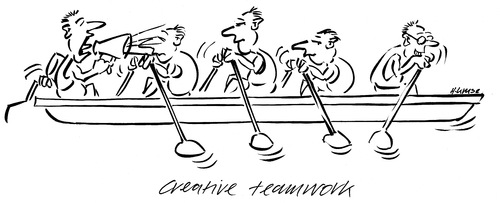
\includegraphics[width=1.00\textwidth]{../figure/creative_teamwork.jpg}
\caption{Capton}
\end{figure}

\subsection{Open Communication}
A team is able to communicate effectively and there is a feeling of open communication between all members of the group. Issues within a team are handled by face-to-face communication. Team members do not talk behind each other's back as there is a respect developed among team members that necessitates direct and open communication on all issues.

\subsection{Decision-Making}
A team has a hierarchy and a built-in decision-making system that helps it to react quickly and effectively to all situations. The members of the group are respected for their various areas of expertise, and the leader of the group has developed the ability to obtain the group members' opinions to formulate the group's response. This applies to decisions made within the group ranging from resolving internal conflict to a potential change in group leadership.

\subsection{Efficient Use of Ideas}

Brainstorming is one way that groups come up with the solution to a problem. An effective team is able to gather information from each member and formulate that information into a response. The team becomes adept at dismissing ideas that will not work, and including effective ideas into what would become the team's solution to an issue.

\section{Contract}

Each team will develop a contract, based on the contract template available in github/Admin. The language that you choose will vary based on your team, but here is an example that you might find useful:

\begin{itemize}
  \item We all promise to listen to each other's ideas with respect.
  \item We all promise to do our work as best as we can.
  \item We all promise to do our work on time.
  \item We all promise to ask for help if we need it.
  \item We all promise to ???.
\end{itemize}

\section{Contribution Documentation}

Each team will develop a method to document your contributions to the overall team effort. Team member contributions will contribute to the grade for this project. The format and methods of documenting the contributions must be decided AND developed before the contract is signed.

\section{Consequences}

Please specify the consequences if the contract rules are broken. Please avoid being punative. Here's an example that you might find useful:

\begin{quote}
If someone on our team breaks one or more of our rules, the team may have a meeting and ask the person to follow our agreement. If the person still breaks the rules, we will ask the professor to help find a solution.
\end{quote}

Follow through with the contract will be reflected in the project grade.

\section{Signatures}

Finally, your contract shall include a signature page with a line for each team member and instructor (based on expectations you have defined outline).

\end{document}
